\section{Basic Attribute-Based Encryption}
In the following sections we will have a look at the different ABE schemes. We will extract the  characteristics of each subtopic of ABE, select a representative candidate and finally, a undertake practical performance comparison to evaluate the scalability is done. 

A suitable candidate in the field of ABE is a scheme that satisfies the requirements stated in section \ref{sec:requirements}. The requirements are a super set of thous defined in \cite{lee2013survey}. For the basic \ac{ABE} schemes we will focus on the requirements \req{C1}, \req{C3}, \req{C5} - \req{C8} and optional requirements \req{O1} and \req{O2}.
The general requirements \req{B1} and \req{B2} will be evaluated by the practical performance and scalability analysis.

Some requirements are left out since not all requirements are directly applicable to all ABE schemes. We need to find the comparable subset of requirements on which bases we are able to compare the schemes. The more we dig deeper into the topic the more requirements can we include in our analysis. 

\subsection{Collusion Resistance (C2 Requirement)}
Lets construct a very basic attribute based encryption scheme to clarify the importance of collusion resistance. Assume a distributed crypto-system based on \ac{RSA}. We setup an \ac{AA} which binds attributes to \ac{RSA} public-private key pairs. The attribute "student" gets bound to $K_{PR(s)}$ for the private key and $K_{PU(s)}$ for the public key. Attribute "works at TU Berlin" gets bound to the key $K_{PK_PR(tu)}$ and $K_{PU(tu)}$ respectively. Now, we setup our very own first ABE scheme. The AA can pin the public keys of each attributes to its public billboard so that every entity in the system can use the public attribute keys for encryption. Each user who is currently a student receives a copy of the private key $K_{PR(s)}$ and each user who is currently working at TU Berlin receives a copy of $K_{PR(tu)}$. 

A user, lets call her for historical reason Alice, wants to share content with all students that are also working at TU Berlin. With our basic scheme Alice is able to use \textit{layered encryption}\footnote{Layered encryption: encrypting a plain text with multiple keys, forcing the decryptor to own all relevant keys} to create an \textit{AND}-policy for her cipher text. She encrypts the plain text $p$ with both public attribute keys $c = K_{PU(s)}(K_{PU(tu)}(P))$ and publishes the ciphertext $c$ to a public CSP so that everyone can download it. Students that are working at TU Berlin owning both private keys can decipher the ciphertext by applying both private keys in reverse order $K_{PR(tu)(K_{PR{s}}(c)}$.

The attentive reader will have notice a crucial security leak in this scheme. This \ac{ABE} scheme is not collusion resistant. In fact, collusion resistance is a core requirement of any ABE scheme. On paper it is defined as the impossibility of any two attribute holder to combine their attributes to archive a higher level of encryption. Lets assume that Bob is a student and Eve is working at \ac{TU}-Berlin. Both users received their private key. Now they can simply exchange their attribute keys so that they are both able to decipher the ciphertext even if they separately do not own both attributes.  

Usually collusion resistance is ensured by issuing each user a private key that is blinded by a random value. This random value will vanish on decryption. However, if two users collude they will mix their blinded values resulting in a plaintext that is still blinded by some unknown value. To ensure collusion resistance pairings are commonly used where a user specific id (\ac{UID}) is generated and bound to the exponent of the user's attribute private key. The decryption method will be designed in that way that the blinding of the attribute private key will vanish. 

\subsection{Boolean Access Formula}
To evaluate if a policy matches given attributes an \textit{Access Tree} or \textit{Linear Secret Sharing Matrix} (\ac{LSSS}) is used. While both representations represent the same boolean formula a \ac{LSSS} is often more efficient. For a better explanation the model of an access tree will be used. For each node of this tree it is evaluated whether the children satisfy a certain condition. This might be implemented as \textit{OR} or \textit{AND} threshold gates. While \textit{OR} can be expressed as $1$-out-of-$n$ children need to satisfy the condition, \textit{AND} conditions are $n$-out-of-$n$ threshold gates meaning all children need to satisfy the condition. This approach is called a monotonic access structure and often referrers to \textit{Threshold Security} or \textit{Threshold Access Structure}. 

\subsection{Key-Policy Attribute-Based Encryption (\ac{KP-ABE})}
In \textit{Key-Policy Attribute-Based Encryption} (\ac{KP-ABE}) \cite{goyal2006attribute}, is a \ac{ABE} technique that associates ciphertexts with attributes that fulfill a policy embedded in the private key assigned to a user. 

The initial paper \cite{goyal2006attribute} did leak some basic requirements that was improved by other work. Such as a fix-length cipher text and attribute revocation. Further, the authors stated that users, once issued a policy, are able to delegate a subset of their access tree to other users. Users them self could act as a new attribute authority to issue other uses a subset of their decryption power. While this is a nice feature for some use cases, in a cloud system the administrator would like to restrict this delegation so that no company external users are able to get company secret keys issued. 
% Further, misbehaving users would like to be able to track traitors selling their private keys for black box decryption.

KP-ABE is meant as a broadcasting encryption scheme used by radio providers so that they can address any user that bought a paid membership to distribute premium content. However, since the policy was bound to the users key it is not possible to address a ciphertext to a specific user group without knowing each users access policy. Only the central authority, which issued the users private keys in the first place, would know who could decipher the encrypted text. This in fact renders \ac{KP-ABE} impractical for the application in a cloud sharing scheme. User would simply don't know who are able to decrypt the cipher text. 

The certainly very specific use case of \ac{KP-ABE} probably led to the circumstances that not much paper using this technique exists. So few that it was hard to find any paper satisfying all requirements previously specified. The only paper that was found implemented direct revocation using negation of attributes \cite{lewko2010revocation}. This would in turn leed to the fact that users private key sizes would grow with each revoked attribute. 

\subsection{Cipher-text Policy Attribute-Based Encryption (\ac{CP-ABE})}
In contrast to KP-ABE stands \textit{Cipher-Text Policy Attribute-Based Encryption} (\ac{CP-ABE}) \cite{bethencourt2007ciphertext}. \ac{CP-ABE} assigns ciphertexts with a policy and user keys with attributes. This enables \ac{CP-ABE} to be much more flexible and verbose in comparison to \ac{KP-ABE}. The big advantage (similar to \ac{KP-ABE}) is that the need for a central authorization server is obsolete. Each ciphertext could simply be accessed by every user and only thous who have the right attribute set present are able to decipher the ciphertext. 

The lack of revocation \req{C8} in \cite{bethencourt2007ciphertext} and the need for a large attribute and user universe was huge \req{C5}. Revocation means that a system manager could revoke attributes from users or even the user himself - in modern company settings an required feature to ensure forward secrecy. Large attribute universe, on the other hand, describes that the number of attributes that can be distributed by the \ac{AA} is so large that it is unlikely that a system will run out of attributes to issue. 

The first proposal of a revocation scheme in \ac{CP-ABE} was in 2010 \cite{liang2010ciphertext}. This scheme used a similar approach like \ac{LKH} to make the revocation process efficient. In 2016 Lui \textit{et. al} \cite{liu2016practical} proposed a revocable \ac{ABE} scheme that supports traitor tracing and large attribute universe. To compare CP-ABE with the other schemes we implemented \cite{liu2016practical}. 

\subsection{Non-Monotonic Access Structure For Attribute-Based Encryption}
While monotonic access structures can describe \textit{AND} or \textit{OR} gates, non-monotonic access structure can also reference \textit{NOT} gates. This adds another layer of find-granularity into the system. In non-monotonic structures, first introduced by Ostrovsky \textit{et. al.} \cite{Ostrovsky:2007:AEN:1315245.1315270}, a user may be excluded from certain topics. 

Take for example Alice who is an intern in the Top Secret company. In monotonic access structure she would receive both attribute private keys: "Intern" and "working in Top Secret Company". By nature of monotonic access structures, she would be able to decipher all content addressed to all employees at the Super Secret company. However, some content might be so confidential that interns shall not be able to access them. This exclusion would not be possible. With non-monotonic access structure an administrator may want to encrypt certain information with the policy "working in Top secret Company AND NOT intern".  

While being an imported field for boolean formula and fine-grand access control domain, non-monotonic access structures did not gain the same attention as \ac{CP-ABE} did. As an candidate which shall represent this \ac{ABE} topic we selected \cite{10.1007/978-3-642-54631-0_16}. With negation of attributes revocation becomes more or less trivial. Each attribute can be versioned and simply excluded on encryption. While this approach is not scalable over time it is simple enough to be implemented in some schemes.   

\subsection{Multi-Authority Attribute Based Encryption (MA-ABE)}
On top of the previous mentioned schemes emerged a new sub topic of \ac{ABE}: \textit{Multi-Authority Attribute Based Encryption} (\ac{MA-ABE}). The main motivation was that a single \ac{AA} is not practically applicable in the real world. Would a single authority administer all attributes, it would also have global decryption power. Take for example the health domain. Here different hospitals need to issue different attribute to their employees. A centralized attribute authority would simply be not able to maintain all the different users. In the real world we face independent domains each maintaining their own non intersecting attribute sets. 

\ac{MA-ABE}, while being a young field of \ac{ABE}, enjoyed, because of the real world relation, a lot of attention in the research area. In addition to the normal requirements like collusion resistance and revocation mechanism \ac{MA-ABE} also deals with the question on how to deescalate the global decryption power of the central authority (\ac{CA}). 

A setup of a \ac{MA-ABE} system looks quite similar over the field of related work. On system initialization we setup the \textit{Central Authority} (\ac{CA}). The purpose of the \ac{CA} is to bootstrap new \textit{Attribute Authorities} (\ac{AA}) which then will administer their own domain. In this domain users and attributes of the \ac{AA} are located. The CA is only used to bootstrap new AAs and assign user their unique identifier. After this is done it could in theory go offline. 

To ensure system wide collusion resistance each user usually gets a unique user identifier (\ac{UID}) assigned. This \ac{UID} is issued by the \ac{CA} which is the only entity having an overview about the whole system. 

A suitable candidate to compare \ac{MA-ABE} to the previous introduced schemes is \textit{Hierarchical Attribute-Based Encryption} (\ac{HABE}, section \ref{sec:HABE}). In short \ac{HABE} is structured around the idea of decryption power delegation. The structure can be imaged like the domain name system. At top level there is the root master administrating the whole system. He can delegate power to sub entities in form of attribute issuing and user registration. This sub entities can again forward a subset of their power to their children. For a complete explanation see \ref{sec:HABE}. We will use \cite{Wang:2010:HAE:1866307.1866414} as representative candidate for \ac{MA-ABE}. 

\subsection{Comparison}
To implement and compare the selected representatives of the different ABE sub topics the charm framework\footnote{\url{http://charm-crypto.io/}} is chosen. Here we can already find implementations for the \ac{KP-ABE} scheme \cite{lewko2010revocation} and for non-monotonic \ac{CP-ABE} \cite{10.1007/978-3-642-54631-0_16}. The other two schemes such as \ac{CP-ABE} \cite{liu2016practical} and HABE \cite{wang2011hierarchical} were implemented  by this work\footnote{\url{https://github.com/Anroc/charm}}. 

\begin{table*}[!ht]
\centering
\begin{tabular}{l 							| l 				| l 						| l }
											& \req{Scheme}		& \req{Security Scheme}		& \req{Expression of access policy}	\\
\textbf{LSW 08}	\cite{lewko2010revocation}	& \ac{KP-ABE} 		& Biliniear maps			& \ac{LSSS}							\\
\textbf{YAHK 14} 
\cite{10.1007/978-3-642-54631-0_16}			& Non-Monotone \ac{CP-ABE} & Binilnear maps 	& \ac{LSSS} Matrix 					\\
\textbf{LW 14} \cite{liu2016practical} 		& \ac{CP-ABE} 		& Binilnear maps 			& \ac{LSSS} Matrix 					\\
\textbf{WLWG 11} 
\cite{Wang:2010:HAE:1866307.1866414}		& Hirachical \ac{CP-ABE} & Binilnear maps 		& \ac{DNF}							\\

\end{tabular}
\caption{Scheme description. }
\label{tab:comparison_baic_abe_overview}
\end{table*}
\begin{table*}[!ht]
\centering
\begin{tabular}{l 	| l					| l 				| l 				| l}
					& \textbf{LSW 08} \cite{lewko2010revocation}	& \textbf{YAHK 14} \cite{10.1007/978-3-642-54631-0_16} & \textbf{LW 14} \cite{liu2016practical} & \textbf{WLWG 11} \cite{Wang:2010:HAE:1866307.1866414} 	\\
\req{C1}			& Yes				& Yes 				& Yes 				& Yes 				\\
\req{C2}			& No				& No 				& No 				& Yes 				\\ 
\req{C3}			& No				& No 				& No 				& No 				\\ 
\req{C4}			& No				& No 				& No 				& No 				\\ 
\req{C5}			& Yes				& Yes 				& Yes 				& Yes 				\\ 
\req{C6}			& - 				& - 				& -					& Yes				\\
\req{C7}			& -					& - 				& - 				& No 				\\
\req{C8}			& Yes				& Yes				& Yes				& Yes				\\
\req{O1}			& No 				& No 				& Yes 				& No 				\\
\req{O2}			& Yes+ 				& Yes+				& Yes				& Yes-				\\
\end{tabular}
\caption{}
\label{tab:basic_abe_comparisons}
\end{table*}

In table \ref{tab:comparison_baic_abe_overview} the main differences of this schemes are listed.  Table \ref{tab:basic_abe_comparisons} shows the requirements and whether they are satisfied by each of the schemes \ref{sec:requirements}. 

Please note that the scheme each address different use cases and were designed with different assumptions and techniques in mind. So the scalability comparison might not be as verbose as a comparison would be, if there was a scheme that exists in all four sub topics of ABE. In our case we selected the schemes that satisfied the most of the requirements for a cloud storage system. 

However, from table \ref{tab:basic_abe_comparisons} it is clear that no scheme fully fulfill all requirements. They reveal a good indicator in which sub topic we should extend our research in. WLWG 11 clearly makes the race here satisfying 6 of 10 of the requirements. 

\req{C6} and \req{C7} could not be satisfied by LSW08, YAHK14 or LW14 since they are not designed with multi-authority support in mind. 
Lets have a look at \req{O2}. LSW08 and YAHK14 both supports fine grant access control by using a \ac{LSSS} access structure. Also both implement non-monotonic access structures which give them the extra plus. LW14, on the other hand, does not support negation of attributes but also uses a LSSS. WLWG11, however, does only support access structures in disjunctive normal form
 (\ac{DNF}) which makes this scheme somehow restricted in expressiveness. 

\begin{figure*}[!ht]
\centering
    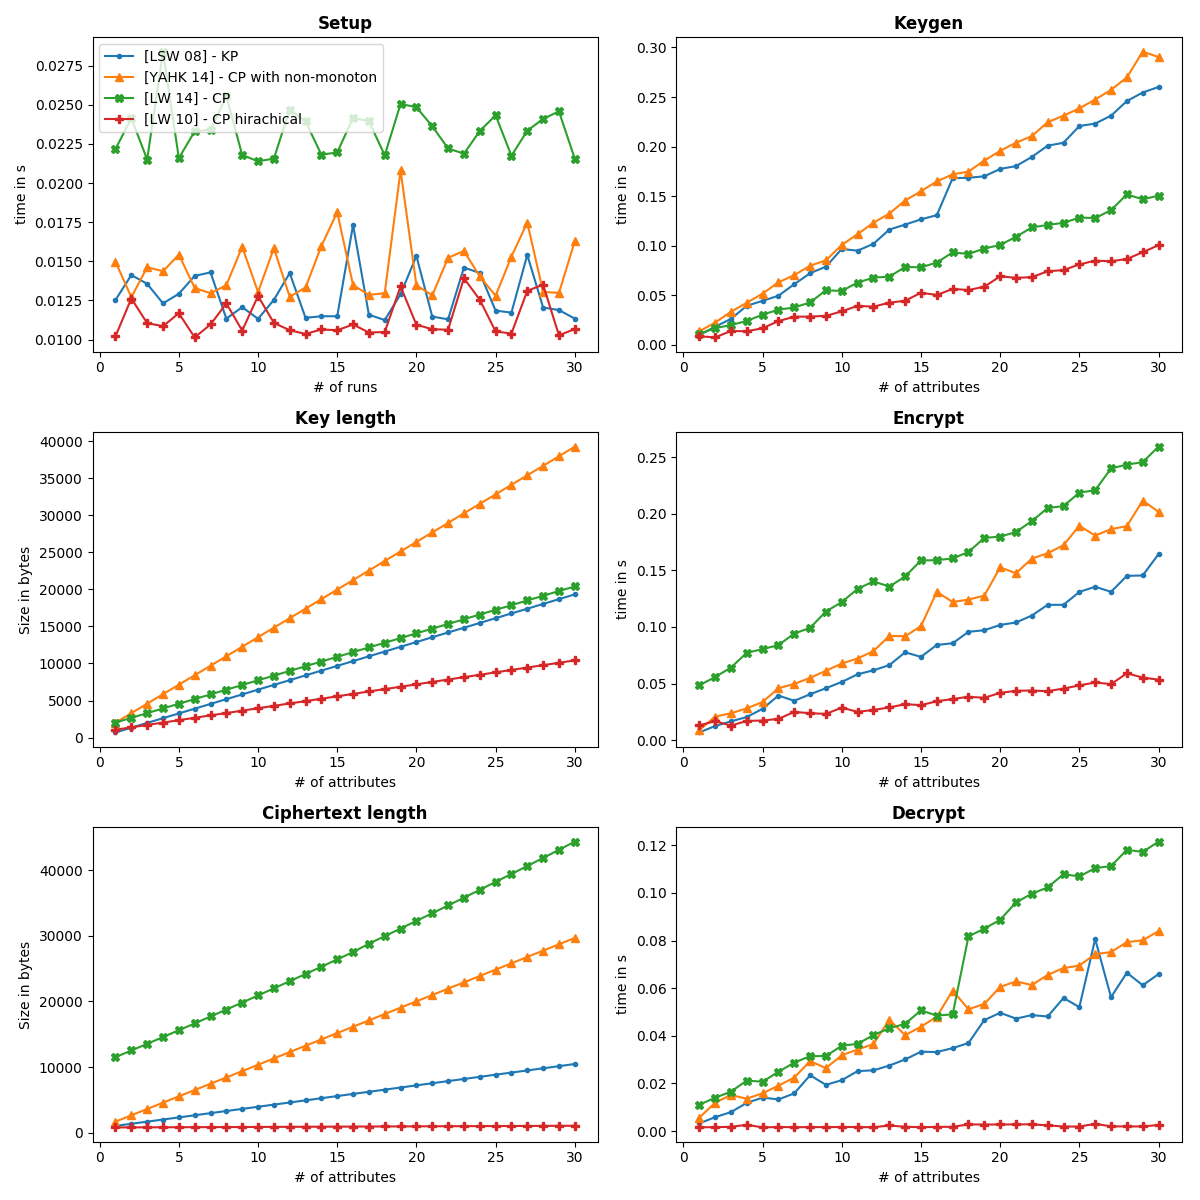
\includegraphics[width=1\linewidth]{img/basic_abe_comparisons.png}
    \caption{Performance and scalability comparison between the chosen schemes with increasing number of attributes. The policy for each new attribute $a_k$ with $a_k \in A$ was defined as $\bigwedge\limits_{a \in A}^a a$. Key generation relates to the creation of users key pairs given an access policy or attribute set.}
    \label{fig:basic_abe_comparison}
\end{figure*}

The  benchmark show in figure \ref{fig:basic_abe_comparison} is executed with a constant size message $m \in G_T$ on a Intel(R) Core(TM) i7-6500U CPU @ 2.50GHz with 16 GB RAM. For the setup was executed 30 times. Here we can see how long the time varies to find suitable curve parameter to initialize the pairing. The other runs are executed with increasing number of attributes. The policy that is used to create the ciphertexts and the user keys in the case of KP-ABE is defined as $\bigwedge\limits_{a \in A}^a a$ where $A$ defines the set of attributes. 

Notable about the comparison in figure \ref{fig:basic_abe_comparison} is that while \ac{KP-ABE} (LSW08) was expected to have the biggest overhead in key generation compared to the \ac{CP-ABE} schemes. This turned out to be not true. It seems more like the time complexity and runtime of the different algorithms surly depends on the design of the scheme. Here we can say that each of the schemes have a linear overhead in runtime. While a constant runtime is only achievable by the HABE scheme the other schemes show a linear time complexity. The HABE scheme in general shows the best overall performance. 
% But it must also be noticed that we specifically excluded attribute authority key generation. 

Due the great performance and the coverage of the most of the requirements of the hierarchical attribute based encryption technique, the field of multi-authority attribute-based encryption will be evaluated in more depth. Regardless of the great scalability of the \ac{HABE} it comes with a non negotiable disadvantage. The root master and the top level domain master have both global decryption power. For each user regardless of the company affiliation the administrator of the system will always be able to decipher ciphertexts of each users. This would break end-to-end encryption. So clearly we would favor solutions that support different attribute authorities so that each company can administer their own domain separately from each other, but we want also that the root, while being able to bootstrap new attribute authorities, is not able to decipher any ciphertext. 